\documentclass{standalone}
\usepackage{pgf-pie}
\usepackage{xcolor}
\usepackage{libertinus}
\begin{document}
\begin{figure}
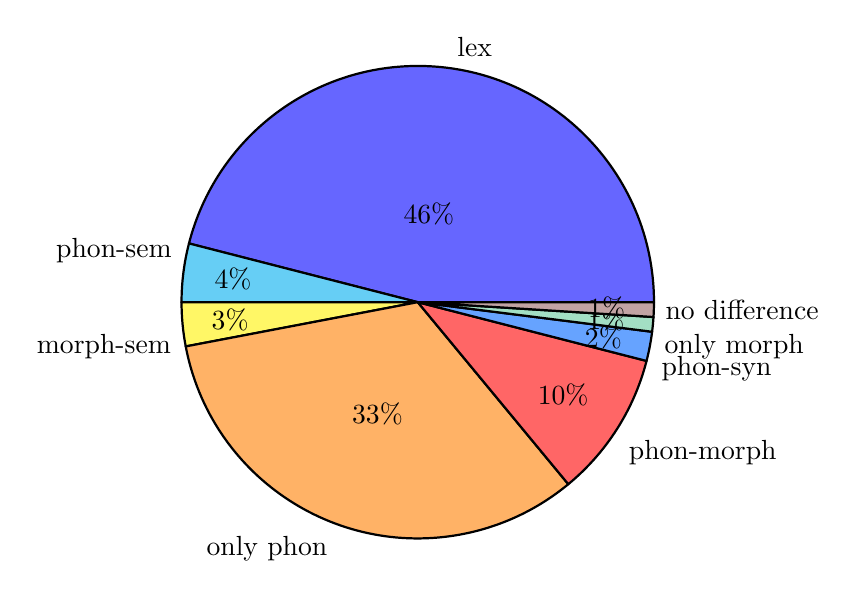
\begin{tikzpicture}
	\pie{46/lex,
		4/phon-sem,
		3/morph-sem,
		33/only phon,
		10/phon-morph,
		2/phon-syn,
		1/only morph,
		1/no difference 
	}
\end{tikzpicture}
\end{figure}
\end{document}
